\chapter{METODOLOGIA}

%Metodologia da bibliografia
\section{Metodologia usada no Levantamento Bibliográfico}


Para atingir os objetivos que orientam este estudo, os procedimentos metodológicos foram idealizados com base em programas educacionais que visam a promoção do empreendedorismo e comportamento empreendedor em cursos de graduação, em instituições de ensino públicas e particulares, como também Startups de natureza educacional.


A metodologia de pesquisa utilizada encontra-se esquematizada na \ref{figura_29}. Buscando construir um levantamento bibliográfico sólido sobre os conteúdos pretendidos neste estudo, foi realizada uma revisão sistemática utilizando como ferramenta o StArt \cite{lapes_start_2016}. A ferramenta StArt foi desenvolvida para apoiar todo processo de Revisão Bibliográfica, por meio de uma árvore hierárquica, categorizando os artigos em proximidade e níveis de aderência às palavras-chave \cite{hernandes_avaliacao_2010}.


\begin{figure}[H]
\centering
\caption{\textbf{Planejamento da pesquisa e construção do portfólio de artigos}}
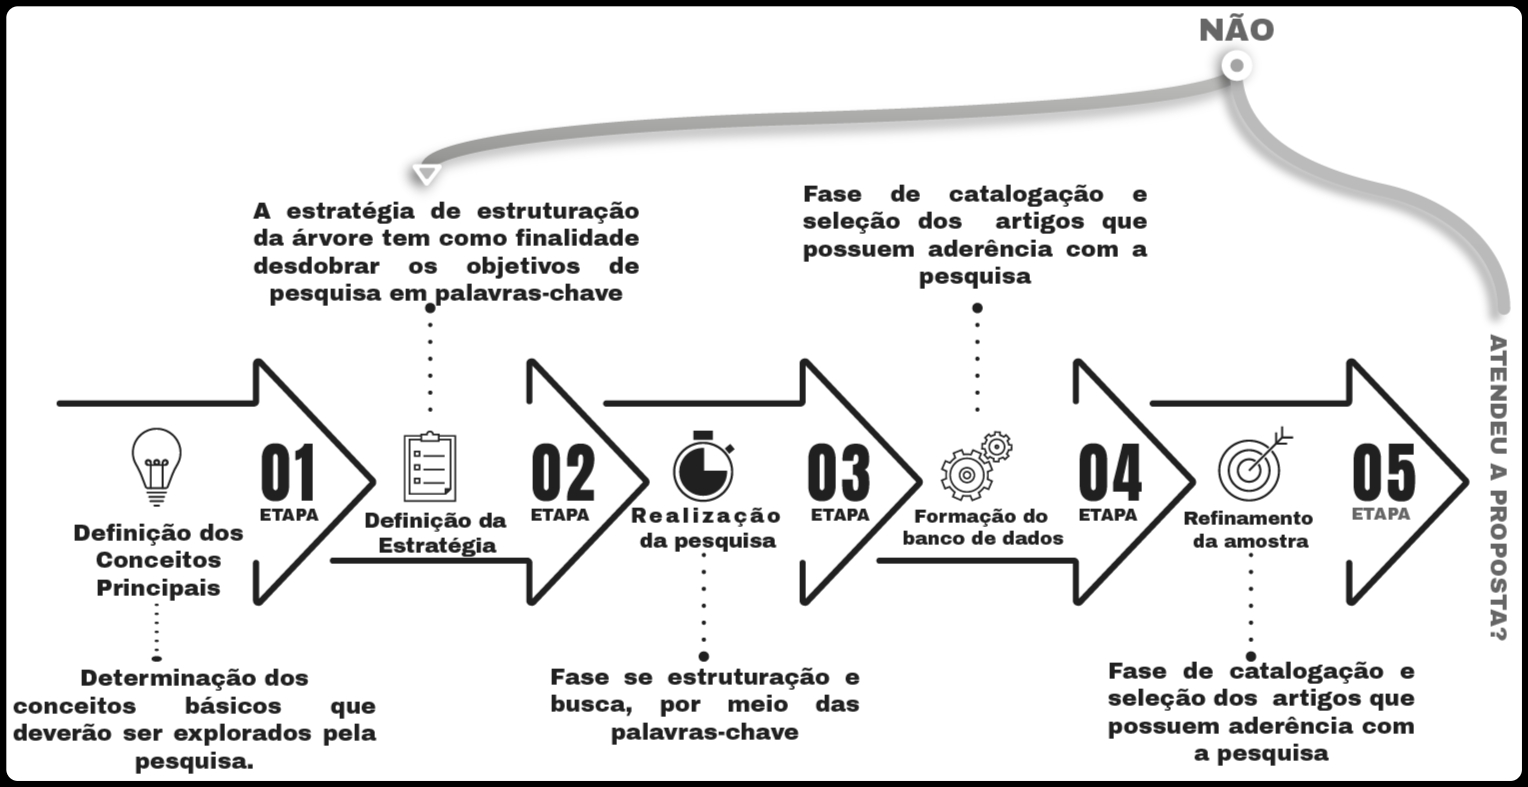
\includegraphics[scale=0.28]{Imagens/fases_pesquisa_bibliografica.png}
\fonte{Adaptado de \citeonline{hernandes_avaliacao_2010}}
\label{figura_29}
\end{figure}

\section{Programa Empreenda AGRO Sustentável: Considerações Metodológicas}


As atividades foram desenvolvidas em quatro encontros \textit{(workshops)}, orientados por metodologias ativas, oficinas, palestras, e ferramentas tecnológicas visando à sinergia entre as estratégias de inovação no uso de tecnologias educacionais e os objetivos da proposta, com vistas a promover aprendizagem significativa e colaborativa, assim como para o aprendizado de ferramentas de gerenciamento e desenvolvimento de negócios.

Durante os módulos do projeto (Workshops), os participantes testaram seus projetos para que novas requisições fossem realizadas e/ou que erros nos planejamentos fossem encontrados e, consequentemente, debatidos e mitigados, utilizando para isso os métodos de modelagem de negócio( \textit{Lean Canvas e Business Model Canvas)} . Após as Sprints (atividades dos três Workshops) serem finalizadas, ou seja, depois que todos os módulos fossem trabalhados, foi iniciado um ciclo de Apresentações e desenvolvimento de habilidades de apresentação e demonstração dos produtos com apresentações (\textit{Pitch}). Destaca-se, ainda, que as inovações capazes de gerar registros de propriedade intelectual, apresentadas nesta pesquisa foram incentivadas para registro e documentação dos direitos.


\section{Planejamento Pedagógico do Programa}

O Programa Empreenda Agro Sustentável traz a proposta do trabalho ao ensino do empreendedorismo de forma multidimensional, multidisciplinar e disciplinado. Tal programa utilizou-se de Oficinas de trabalho particionados em temas que permitissem a compreensão global do empreendedorismo, enquanto admite o ser humano como um ser multidimensional e culturalmente contextualizado no desenvolvimento de um negócio inovador.

A proposta do programa foi combinar oficinas que visam o desenvolvimento das características negociais e seus planos com palestras ministradas por profissionais de alto conhecimento nas áreas específicas de um negócio escalável. Com a aprendizagem baseada em equipes \textit{(team-based learning)} o programa delimitou inicialmente a inscrição dos participantes somente em grupos pré-estabelecidas, de modo a ter como iniciativa, maiores afinidades durante o desenvolvimento dos trabalhos.


\subsection{Mobilização das Equipes}

Inicialmente fez-se abertas vagas para estudantes do curso de graduação, ligadas aos cursos de Ciências Agrárias da Universidade Federal de Sergipe-UFS, onde as inscrições foram realizadas por equipe, desde que os alunos inscritos apresentassem os seguintes critérios:

	
\begin{itemize}
\item{Estarem regularmente matriculados e cursando quaisquer dos cursos e ao menos um aluno ligado as ciências agrárias;}
\item{Comprovarem disponibilidade de tempo para participação em todas as oficinas programadas;}
\item{Lidar com trabalhos em equipe.}
\end{itemize}

Trabalhou-se com \textbf{118 alunos} participantes efetivos no programa, o qual será considerado o número de amostra para a pesquisa. Para delimitação das equipes foram elencadas 12 cadeias produtivas  prioritárias e áreas de desenvolvimento agrário destacando-se:

\begin{multicols}{2}
\centering
    \begin{itemize}
    \item{Agricultura Sustentável;}
    \item{Alimentos;}
    \item{Aplicações Mobile}
    \item{Automatização Agrícola}
    \item{Biotenologia}
    \item{Economia Criativa}
    \item{Fitoterapia}
    \item{Higiene/Produtos de beleza}
    \item{Turismo}
    \item{Pecuária Verde}
    \item{Tecnologias gerais}
\end{itemize}
\end{multicols}



Com a finalidade de propor uma melhor mentoria no desenvolvimento dos objetivos propostos, o programa foi desenvolvido as quatro oficinas de trabalho definidas nesta pesquisa como  "Workshops" (Figura \ref{figura_17}), que abordaram temas pertentes ao empreendedorismo e o comportamento empreendedor, a saber:

\begin{itemize}

\item {1º Workshop \textbf{Insight e despertar}: O que é startups, empreendedorismo, comportamento empreendedor e cultura empreendedora, problemas (segmentação do mercado), segundo os Objetivos do Desenvolvimento Sustentável (ODS), Modelagem do negócio e Criatividade;}
\item {2º Workshop \textbf{Ideação}: A busca de oportunidades como característica empreendedora, construção do \textit{\textit{Lean Canvas}}, mapa de empatia, validação da proposta de valor, economia colaborativa e \textit{coworking};}

\item {3º Workshop: \textbf{Hackathon}: Prototipagem para o MCVP, O que você pode fazer por seu cliente e como o cliente adquire seu produto?;}

\item {4º Workshop \textbf{Demoday}: Destaca-se que o mecanismo de pesquisa que foi utilizado neste experimento foi composto por cinco blocos de questões de múltipla escolha baseadas principalmente em escalas de cinco ou sete possibilidades.}
\end{itemize}

\subsection{1º Workshop}

Buscando um engajamento maior dos participantes foram aplicadas cinco estratégias/dinâmicas: Apresentação das ideias propostas inicialmente; Círculo Dourado; Quem sou eu no Universo?; Descoberta do cliente usuário e o  desenvolvimento da proposta de valor (Figura \ref{figura_30}).

\begin{figure}[!h]
\centering
\caption{\textbf{1º Workshop Empreenda Agro Sustentável}}
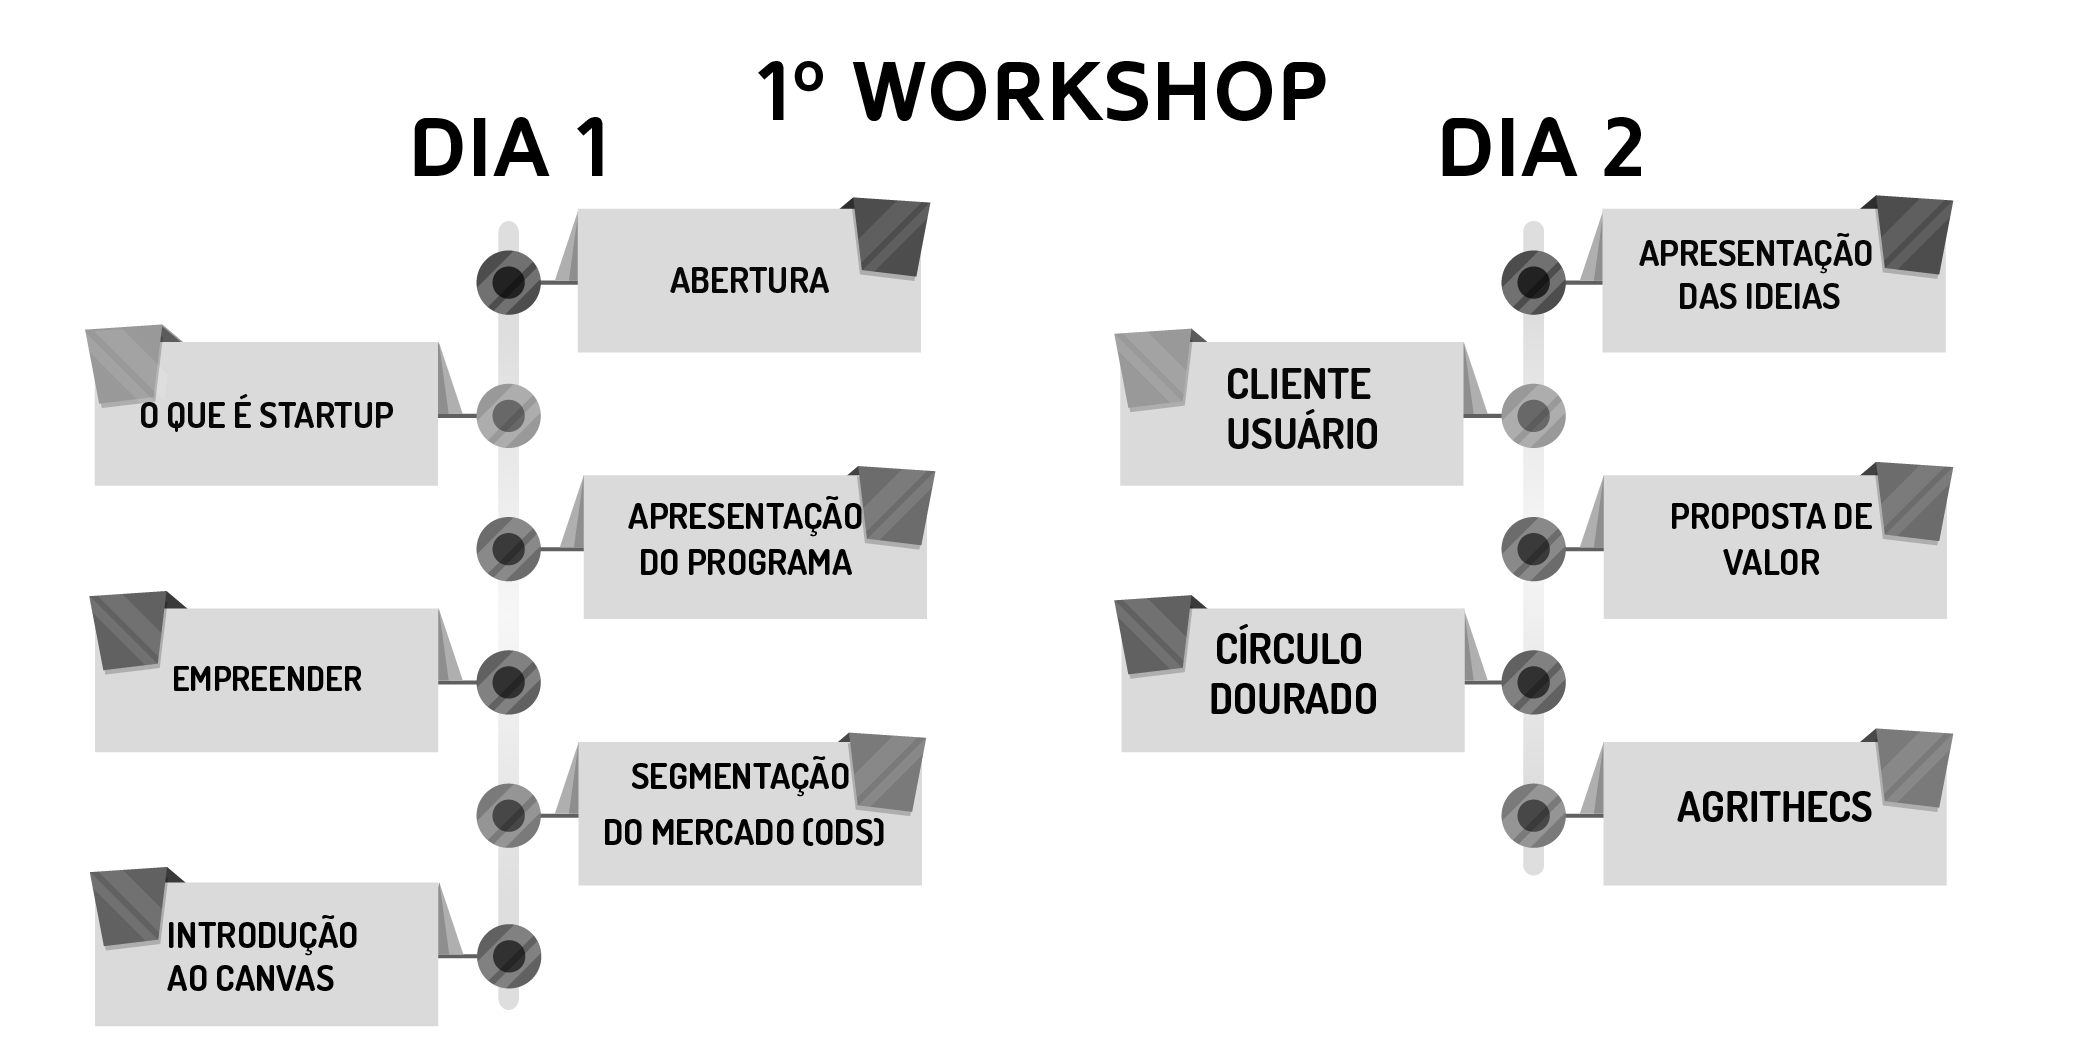
\includegraphics[scale=0.3]{Imagens/workshop-01.png}
\fonte{O Autor}
\label{figura_30}
\end{figure}
%\newpage

A dinâmica \textbf{"Apresentação das ideias propostas"}\ visou a construção de um panorama visual de todos os insights, inscritos no programa, como também as temáticas mais buscadas pelos alunos. As atividades de Expressão Oral (EO) oportunizam aos estudantes a apropriação de recursos linguísticos e interativos inerentes às práticas orais e considerando que a EO pode ser uma eficaz ferramenta para o ensinamento de conteúdos conceituais, procedimentais e atitudinais em contato social \cite{baltar_genero_2010}.

A atividade proposta, considera que a expressão oral mesmo que incipiente proporciona aos alunos o exercício da criticidade, abordar e levantar seu ponto de vista e seus interesses na participação do programa, podendo executar a sua verve crítica, enquanto possibilita o aprimoramento das atitudes discursivas durante a argumentação. O estudante torna público suas expectativas e se compromete informalmente com a comunidade de desenvolver suas propostas.

A segunda dinâmica \textbf{Golden Circle} (Cícrulo Dourado) desenvolvido por \citeonline{sinek_golden_2015} tem por objetivo: criar ou desenvolver o valor de um novo produto, ideia ou negócio, tal dinâmica é pautada em três pilares: O quê, Como e Porquê. O Círculo Dourado e formado por três círculos de diferentes tamanhos que se completam. Ao centro está o \textbf{Porquê}, que objetiva a expressão do real propósito do negócio pensado pelo grupo. Este Refere-se ao conjunto de iniciativas e compromissos pensados para escalar e promover aos usuários e clientes o valor que a Startup realmente acredita. Resumidamente é o que a empresa de fato acredita ser o  diferencial perante a concorrência e ao mercado atual, este é o ponto de partida da dinâmica.


\begin{figure}[H]
\centering
\caption{\textbf{Golden Circle}}
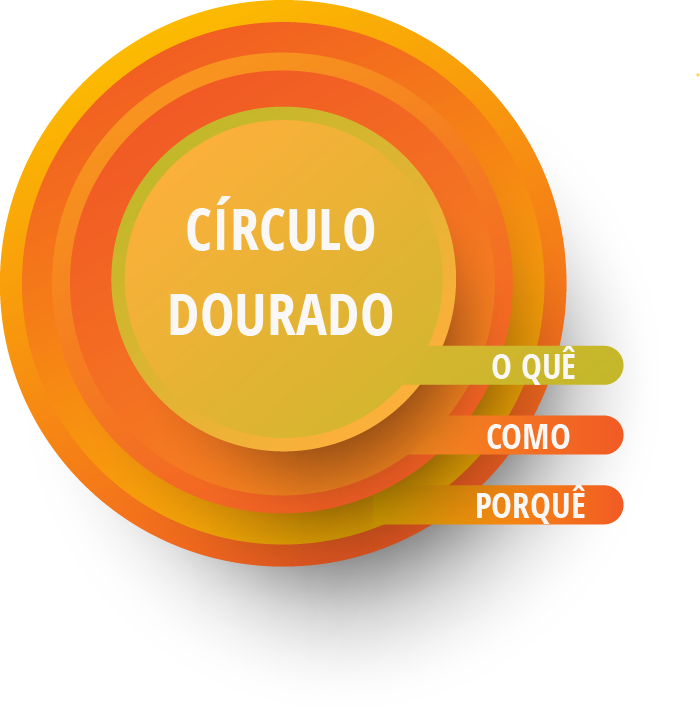
\includegraphics[scale=0.25]{Imagens/circulo_dourado.png}
\fonte{Adaptado de: \cite{sinek_golden_2015}.}
\label{figura_5}
\end{figure}
%\newpage

\subsection{2º Workshop}

Tendo a perspectiva macro do que venha a ser inovação e meios de negócios, o segundo encontro apresentou a proposta de descoberta de oportunidades e desenvolvimento do insight, por meio da busca de hipóteses de negócios e mineração de inovações (Figura \ref{figura_31}).




\begin{figure}[H]
\centering
\caption{\textbf{2º workshop Empreenda Agro Sustentável}}
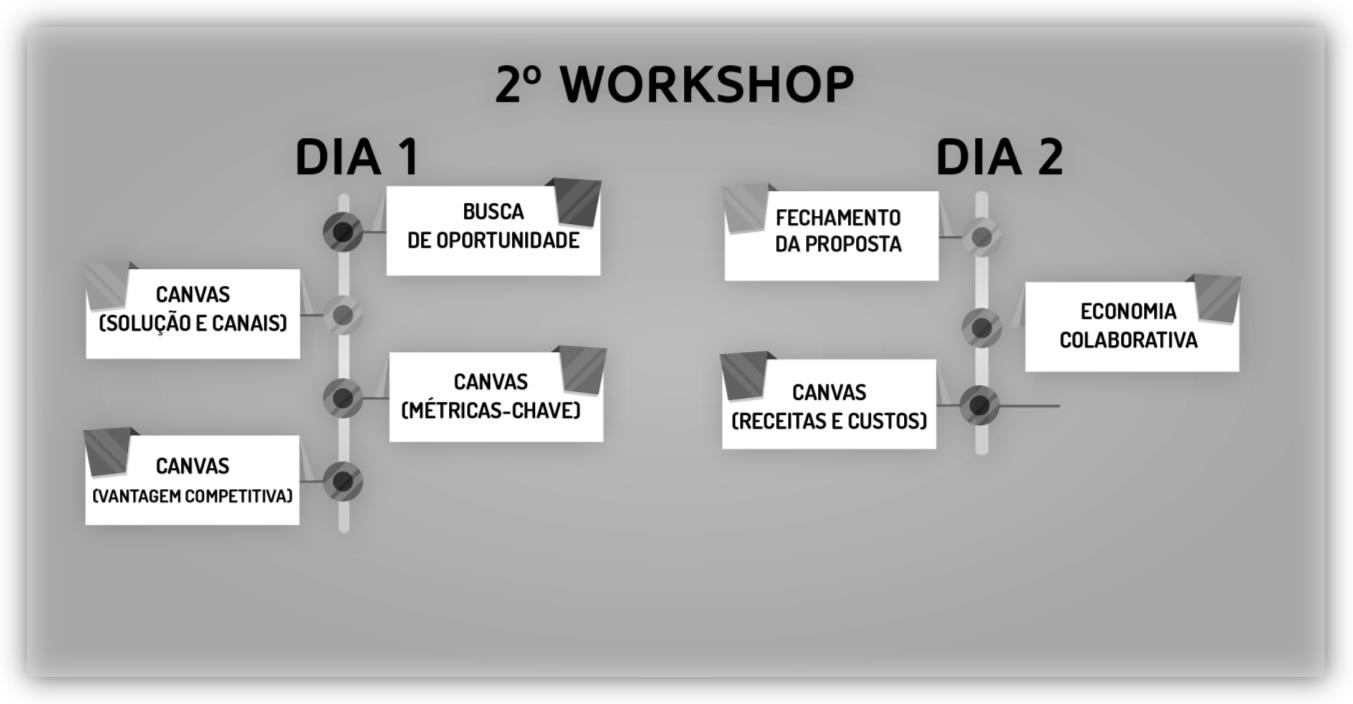
\includegraphics[scale=0.3]{Imagens/workshop-02.png}
\fonte{O Autor.}
\label{figura_31}
\end{figure}

Foi construído o Mapa de empatia de modo a compreender os desejos e necessidades dos clientes e usuários até mesmo seu estado emocional, que influenciará nos seus anseios, e na aquisição de produtos e serviços. Esta necessidade de entender e assimilar as necessidades dos usuários é prioridade no atendimento das expectativas dos usuários. É um ponto fundamental para que as unidades de informação trabalhem orientadas à qualidade e com possibilidade de incorporação de serviços inovadores \cite{valdrich_mapa_2018}. O mapa de empatia é uma ferramenta visual para conduzir esta descoberta, ele é composto por 6 (seis) reflexões diferentes sobre o cliente, são elas: \textbf{as dores}, \textbf{os ganhos},\textbf{o que ele escuta}, \textbf{o que ele vê}, \textbf{o que ele pensa e sente} e \textbf{o que ele faz}, é possível entender o mapa de empatia por meio da Figura \ref{figura_6}.

\begin{figure}[H]
\centering
\caption{\textbf{Exemplo do Mapa de empatia}}
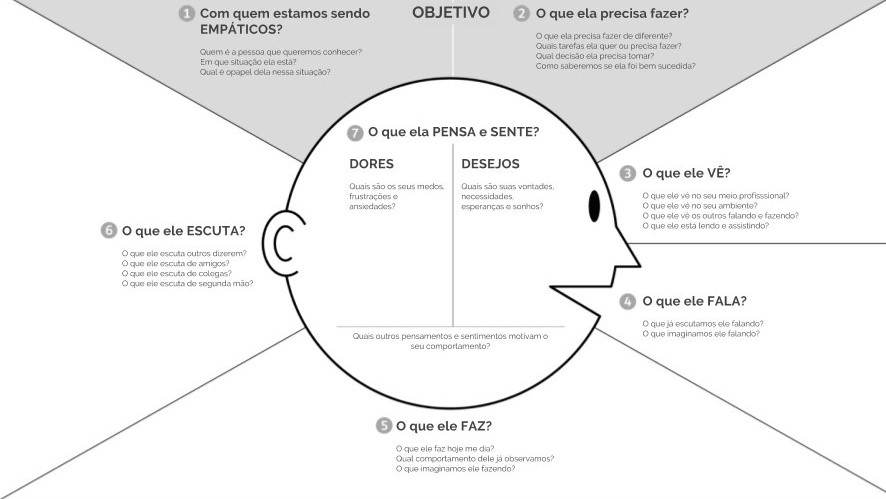
\includegraphics[scale=0.5]{Imagens/mapa_empatia.jpg}
\fonte{\cite{osterwalder_value_2019}.}
\label{figura_6}
\end{figure}


Após o desenvolvimento da ideia da Startup por meio do mapa de empatia, é esperado que o participante tenha uma visão holística do que deseja produzir como negócio, assim para que sejam visualizadas as possibilidades e estruturas do negócio. Será trabalhado o quadro (ferramenta) \textit{Lean Canvas} proposto por Ash Maurya, tendo como base para o desenvolvimento o \textit{Business Model Canvas} (BMC) entre outros materiais. Ele adaptou 4 quadros do BMC, buscando trabalhar aspectos de maior risco na criação de Startups \cite{maurya_running_2012}. Ele é ideal para o quando o negócio está no começo ou ainda não deu início às atividades e que ainda não fez testes sobre suas estruturas comerciais. Essa é a hora de analisar de maneira mais aprofundada os problemas que o mercado apresenta e estruturar de uma forma melhor a solução oferecida pela startup, encontrando aí o melhor resultado nessa equação \cite{sebrae_aprenda_2019}. O quadro é comporto pelos seguintes campos: \textbf{1.\textsuperscript{o} Problema, 2.\textsuperscript{o} Segmentos de Clientes, 3.\textsuperscript{o} Proposta Única de valor, 4.\textsuperscript{o} Solução, 5.\textsuperscript{o} Canais, 6.\textsuperscript{o} Fontes de Receitas e 7.\textsuperscript{o} Estrutura de Custos}.

O problema deve ser as dificuldades que a startup deve resolver por seus usuários. O segmento de Clientes deve prever quais os clientes e usuários da sua startup. De que forma eles podem ser segmentados? O que torna o seu produto diferente e merecedor do dinheiro dos clientes? e o que de fato a startup tem a oferecer ao cliente/usuário. No campo (Solução) o aluno explicou o menor conjunto de funcionalidades de seu produto, de que forma ele vai entregar a proposta de valor anteriormente pensada.

Ao chegar nas métricas chaves eles projetam como será a geração de capital deste negócio ou de que forma reterão seus clientes/usuários, no campo (Canais), será descrito uma lista de meios de “marketing” e captação de cliente. Para a estrutura de custos, os participantes descreveu-se todos os gastos sendo custos fixos e variáveis de seu negócio. Para o Fluxo de Receita ele identificará qual o modelo de receita — assinatura, anúncios, \textit{freemium}, e determine as premissas para indicadores como "Life time value", etc. Por fim, na vantagem competitiva deve ser explicado o algo que não pode ser comprado ou copiado, deve ser de fato a inovação de seu negócio,  \cite{maurya_running_2012, sebrae_aprenda_2019}. É recomendável a construção do quadro seguindo esta sequência, e na Figura \ref{figura_7} é visualizado o quadro que foi utilizado durante o programa.



\begin{figure}[h!]
\centering
\caption{\textbf{Diagrama do Modelo  \textit{Lean Canvas} do Programa Empreenda Agro Sustentável}}
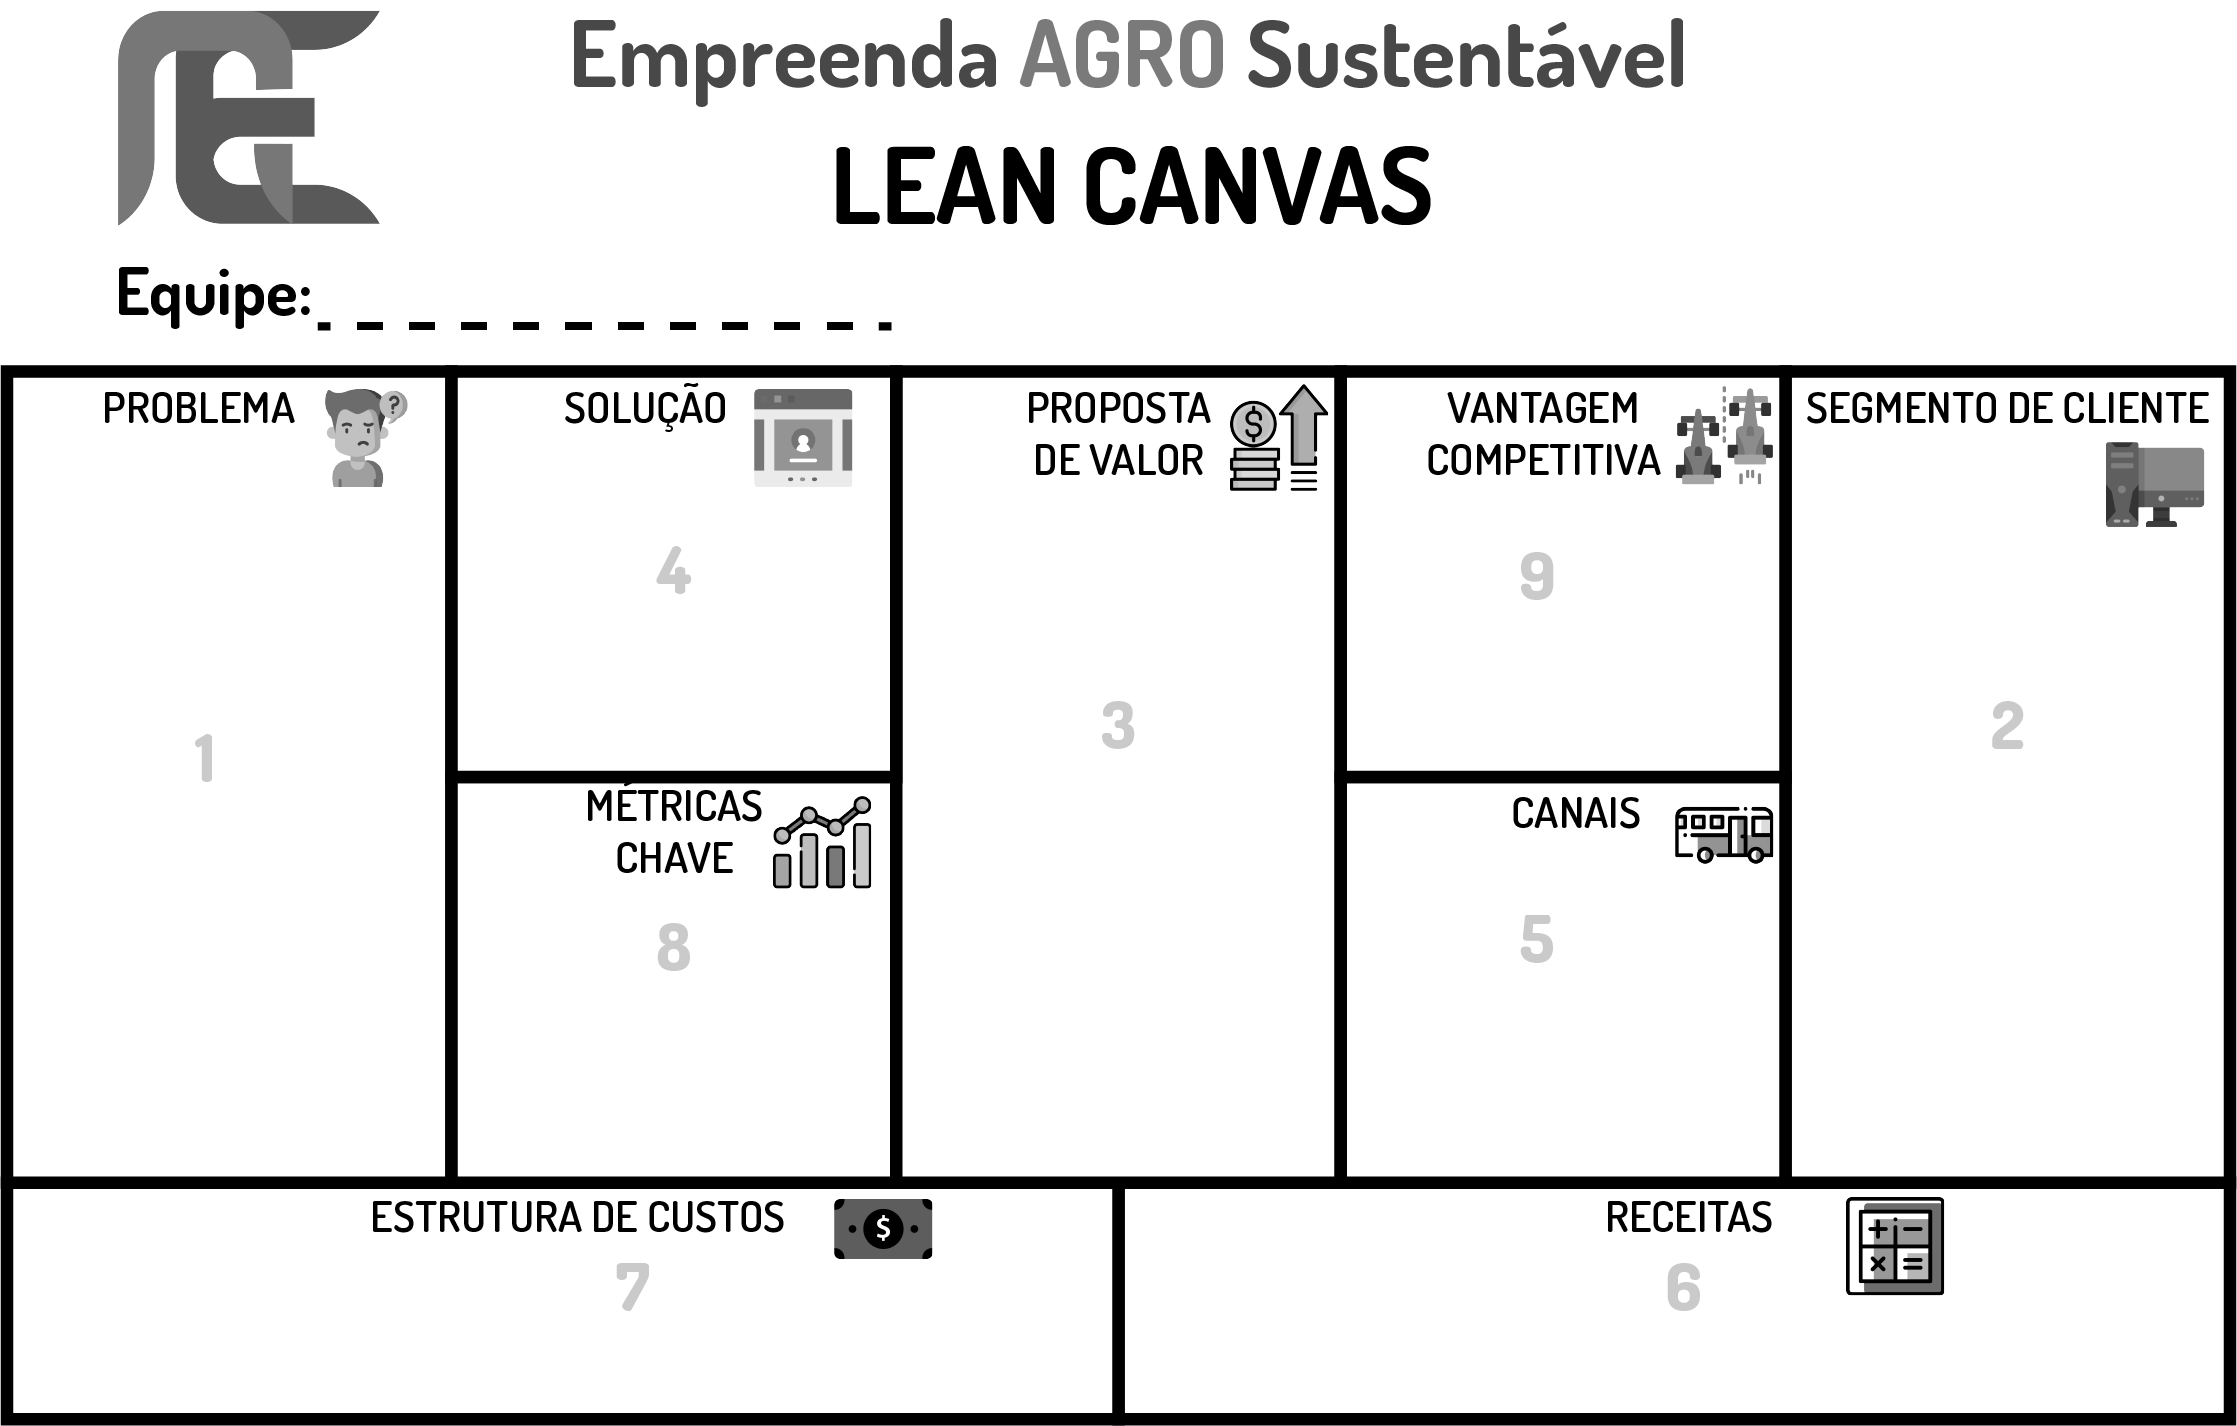
\includegraphics[scale=0.9]{Imagens/canvas.png}
\fonte{O autor.}
\label{figura_7}
\end{figure}


\subsection{3º Workshop}
 
Nesta Oficina de trabalho (“Workshop”) foi trabalhado o Hackathon, momento no qual os alunos desenvolveram de forma prática o seu Mínimo Produto Comercialmente Viável (MVBP sigla em inglês), que segundo \citeonline{aulet_empreendedorismo_2019}.o MVBP é um produto completo o bastante para que um cliente possa ganhar valor com ele, o qual deva possibilitar a demonstração concreta do que se pretende oferecer (Figura \ref{figura_32}).

\begin{figure}[H]
\centering
\caption{\textbf{Hackathon Empreenda Agro Sustentável}}
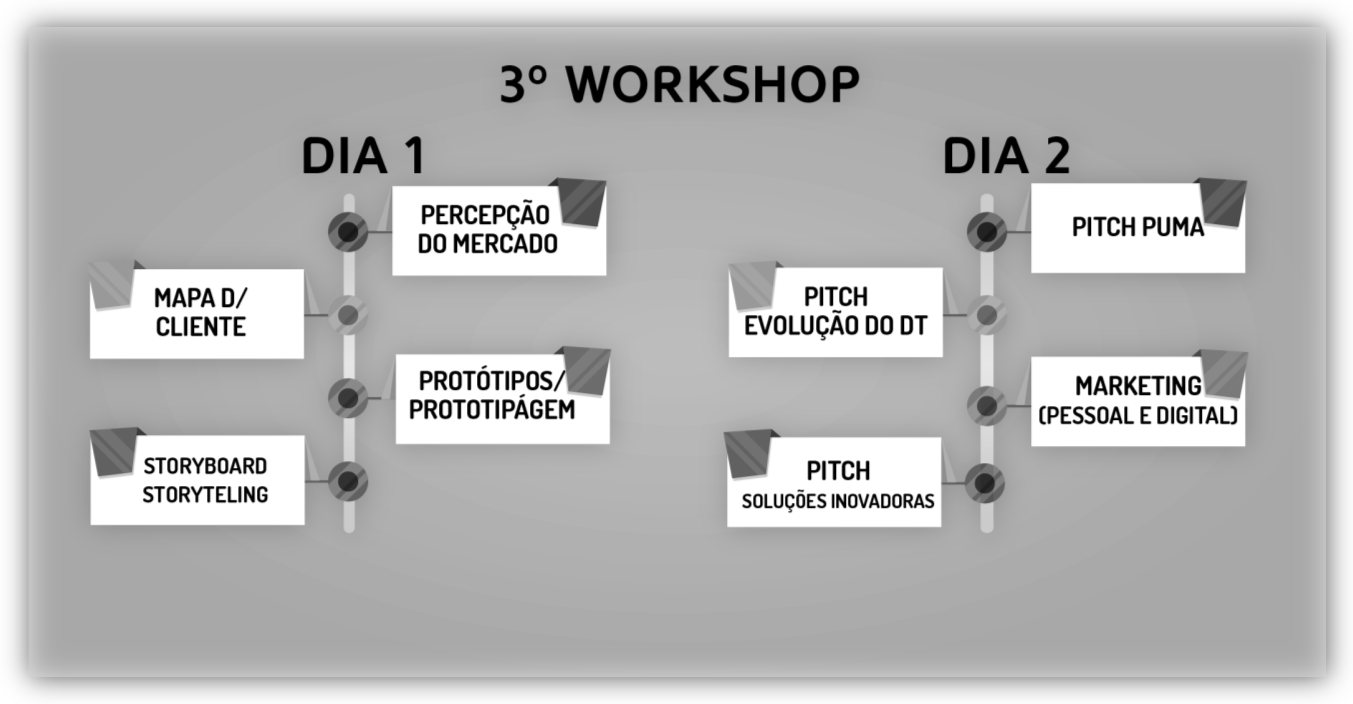
\includegraphics[scale=0.3]{Imagens/workshop-03.png}
\fonte{O autor.}
\label{figura_32}
\end{figure}

\subsection{4º Demoday}

O Demoday ou Dia de Demonstração dos modelos de negócios das startups foi realizado no dia 22 de novembro de 2019. Esse foi o evento em que as startups se apresentaram para investidores, que são representados por ventures capitals, aceleradoras ou investidores-anjos. Nessa oportunidade os jovens empreendedores apresentaram seus projetos em busca de investimentos. As startups formadas pelo programa realizaram a exposição e apresentação de seus modelos de negócio e protótipos, bem como a apresentação dos pitchs de cada equipe para o público presente que buscou cada bancada, além de participação em um “Talk Show” com mais uma exibição de pitchs para todo público presente no evento (Figura \ref{figura_33}).

\begin{figure}[H]
\centering
\caption{\textbf{Demoday Empreenda Agro Sustentável}}
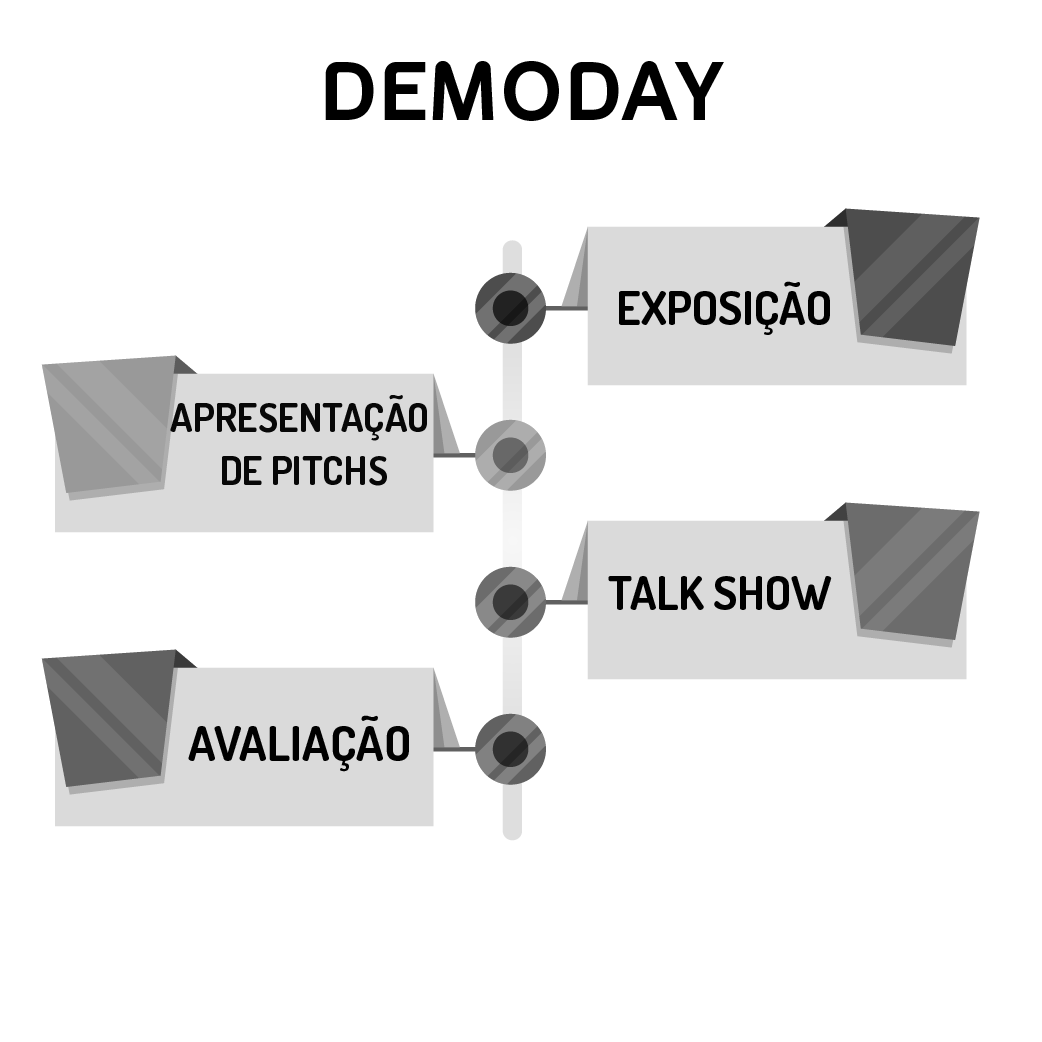
\includegraphics[scale=0.2]{Imagens/workshop-04.png}
\fonte{O autor.}
\label{figura_33}
\end{figure}

\section{Questionário para Análise de Campo}

A utilização de um método de pesquisa em uma dissertação depende da escolha de um modelo mais adequado ao problema do estudo e aos objetivos pretendidos. Assim, esta pesquisa foi desenvolvida com caráter descritivo tendo como base o método de pesquisa \textit{Survey} exploratório-descritivo, uma vez que este método busca contribuir para o conhecimento geral de uma área particular de interesse, pois, envolve uma coleção de informações de indivíduos através de questionários e entrevistas sobre suas atividades ou sobre si mesmos  \cite{forza_survey_2002}. Na Figura \ref{figura_8} é possível compreender as fases do \textit{Survey} exploratório-descritivo.


\begin{figure}[H]
\centering
\caption{\textbf{Fases do \textit{Survey} exploratório-descritivo}}
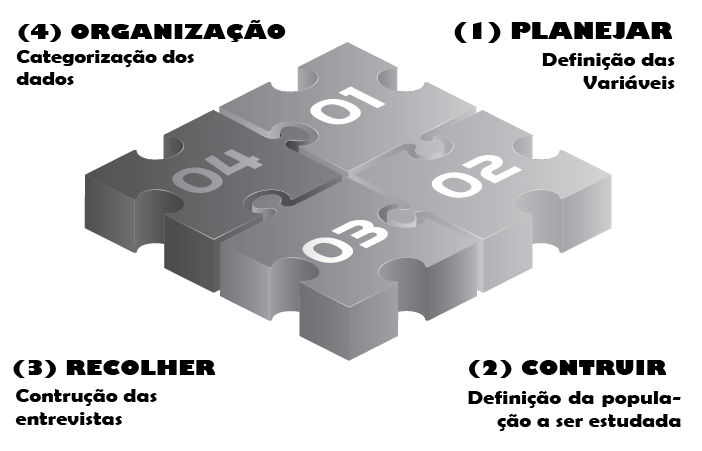
\includegraphics[scale=0.5]{Imagens/survey.png}
\label{figura_8}
\fonte{Adaptado de \cite{moser_survey_2017}.}
\end{figure}


O questionário apresenta 5 conjuntos de questões dos mais diversos contextos relacionados ao empreendedorismo, medindo diferentes elementos do empreendedorismo e comportamento empreendedor no meio educacional tanto vindo dos discentes quanto dos docentes. O instrumento de pesquisa que foi utilizado neste experimento foi composto por Cinco blocos de questões de múltipla escolha baseadas principalmente em escalas de cinco ou sete possibilidades.

As perguntas iniciais têm por objetivo de traçar o perfil dos alunos entrevistados, tais como: gênero, faixa etária, curso vinculado e o delineamento de interesse nas áreas de ensino ligadas ao empreendedorismo sustentável tal questionário foi baseado nos experimentos desenvolvidos por \citeonline{lima_educacao_2014}.

Primeiro bloco contendo 11 questões abordou a ligação da família e o apoio familiar no empreendedorismo, tendo como alternativas, “Discordo totalmente” a “Concordo totalmente”.

O Segundo conjunto foi composto por 7 questões que analisam a intenção empreendedora do aluno, tendo como alternativas, “Discordo totalmente” a “Concordo totalmente”.

O Terceiro conjunto tratou sobre os interesses dos alunos por disciplinas e atividades relacionadas ao empreendedorismo.

O Último conjunto foi composto por 10 questões relacionadas a autoeficácia e a intenção em ter sua própria empresa ou ser autônomo, e foi composto por questões de múltipla escolha partindo da alternativa “Completamente Inseguro” a “Completamente Seguro”. A Figura  apresenta o universo das dimensões que serão conduzidas nesta pesquisa.


Desta forma a pesquisa caracteriza-se como uma pesquisa de levantamento do tipo exploratório-descritivo sob corte Longitudinal, que segundo \citeonline{tormen_potencial_2005} ela se destaca por compreender uma amostra expressiva em relação ao universo pesquisado.

\section{Universo da Pesquisa}

O universo desta pesquisa é composto por \textbf{1227 discentes} matriculados nos cursos de graduação do centro de Ciências Agrárias Aplicadas CCAA da Universidade Federal de Sergipe (UFS), campus São Cristóvão \cite{andrade_ufs_2019}. É importante considerar que esta pesquisa não considerou classe social local de ensino anterior, e desempenho acadêmico do aluno durante a graduação.

\section{Tamanho da Amostra Utilizada}

Muitas vezes não se faz necessário, ou não é possível, dispor de toda a população objetivo do projeto. Desta forma é necessário dispor de uma parte do universo da pesquisa para que seja possível realizar inferências confiáveis da população total \cite{marino_manual_2003}.

Para que fosse possível a análise populacional de forma fidedigna, foi selecionada uma amostra de tal população. Amostra é o número de pessoas que serão entrevistadas nesta pesquisa. Esse número foi inicialmente considerado como o número máximo de capacidade de condução efetiva do programa, partindo do universo pesquisado (CCAA) que era de\textbf{1227 discentes}.


Considerando este valor como população do universo pesquisado, 95\% (Z =1,96) para o valor médio que aceitaríamos para alcançar o nível de confiança desejado segundo a distribuição de Gauss, admitindo também a margem de erro máximo de 0,5\% foram abertas 300 vagas, destas foram preenchidas \textbf{118}, e assim esta pesquisa apresenta uma \textbf{margem de erro de 8,57\%}.

\section{Tratamento dos Grupos de Itens do Questionário Aplicado: Autoeficácia, Intenção Empreendedora, Apoio Familiar}

A constatação da não-normalidade dos dados se deu quando analisadas as questões resultantes da primeira aplicação para todos os cursos, sendo observado o valor de probabilidade abaixo do nível de significância de 0,05. Uma vez constatada a não normalidade dos dados amostrais, esses dados também passaram a ser tratados de forma não-paramétrica, buscando métodos para análise deste perfil.

Foi realizada Análise Fatorial, para destacar a consistência interna dos resultados obtidos durante o primeiro questionário, objetivando a exclusão de dados com consistência inferior aos demais resultados apresentados \citeonline{damasio_uso_2012}.

O teste KMO (\textit{Kaiser-Meyer-Olkin Measure of Sampling Adequacy}), da Análise Fatorial, testa se os dados estão suficientemente ligados para que se possa proceder a análise. Desta forma, este método foi utilizado para validação do questionário.

O Teste de Kolmogorov-Smirnov K-S foi utilizado para avaliar a aderência dos valores das variáveis quantitativas contínuas à distribuição normal. A partir dos resultados deste teste, foi possível decidir se seriam utilizados os testes paramétricos ou não-paramétricos.

\section{Análises Estatísticas do Survey}


Por haver pequenas adaptações do GUESSS a este experimento, foi realizada uma análise fatorial e de variância multivariada (análise de fatores ortogonais, com rotação Varimax), já que, uso destes métodos facilita na aglutinação dos fatores por similaridade \cite{hair_multivariate_2006}. Esta pesquisa considera quatro conjuntos de variáveis aglutinadas que influenciam na natureza da resposta empreendedora. Diversos autores abordam diferentes pontos sobre esta temática, visto que este programa se comporta como uma fase de pré-aceleração, quando são abordados os fatores que podem ter comportamento de conjunto de variáveis independentes, quando submetidas à participação dos alunos no programa. A Figura \ref{figura_9} representa as 4 dimensões estudadas:


\begin{itemize}
\item {Interesse em conteúdos relacionados a educação em empreendedorismo;}
\item {Dimensão da Autoeficácia dos estudantes;}
\item {Dimensão da participação familiar e influência de terceiros no desenvolvimento empreendedorismo;}
\item {Dimensão e intenção  ao empreendedorismo dos estudantes;}
\end{itemize}



\begin{figure}[H]
\centering
\caption{\textbf{Dimensões estudadas}}
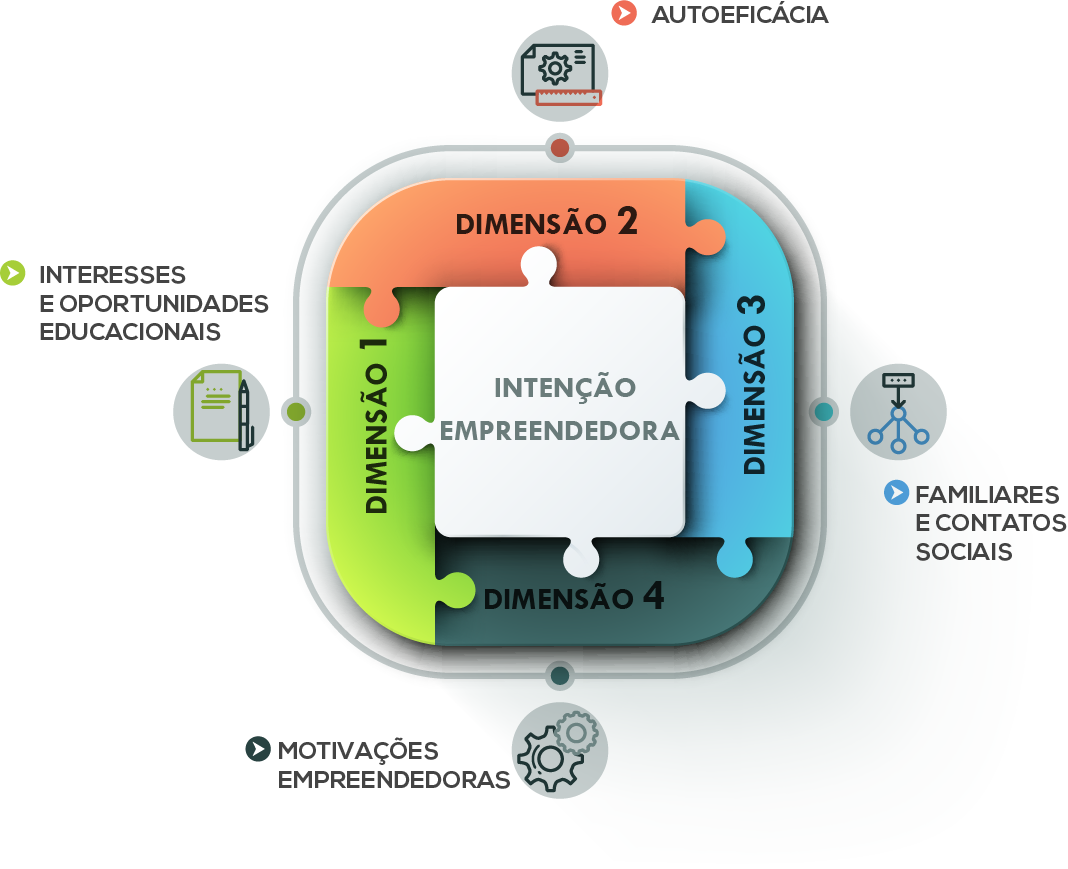
\includegraphics[scale=0.15]{Imagens/dimencoes.png}
\fonte{O autor}
\label{figura_9}
\end{figure}



Já para analisar a aderência dos resultados do questionário proposto \textbf{Interesse em conteúdos relacionados a educação em empreendedorismo;} após a participação no programa, foi utilizado um teste de \textit{Kolmogorov-Smirnov} uma vez que os dados satisfazem as exigências para tal teste. O K-S é um teste não paramétrico sobre a igualdade de distribuições de probabilidade contínuas e unidimensionais que pode ser usado para comparar uma amostra com uma distribuição de probabilidade de referência ou duas amostras uma com a outra. Ele tem por objetivo verificar diferenças de grupos de variáveis categóricas (independentes) quanto aos seus impactos sobre diversas variáveis métricas (dependentes) em paralelo \cite{hair_alise_2009}. Após observar a aderência, existe diferença significativa entre as respostas obtidas no questionário. Desta forma foi aplicado o teste post-hoc \textit{Mann Whitney}, que se mostra como sendo uma rotina não paramétrica do teste T-studant para amostras independentes. O teste é baseado nos postos dos valores obtidos combinando-se às duas amostras. Isso é feito ordenando-se esses valores, do menor para o maior, independentemente do fato de qual população cada valor provém \cite{matsouaka_optimal_2018}.

Este modelo aplica-se a esta pesquisa, pois, ela tem por objetivo avaliar as alterações quanto ao perfil empreendedor em grupos de alunos participantes do Programa de extensão Empreenda Agro Sustentável. Desse modo, é possível avaliar se as diferenças entre os níveis médios dos grupos captados pela \textit{survey} são significativas entre os grupos e dentro dos grupos \cite{rocha_avaliacao_2014}.

A hipótese aqui apresentada será utilizada para condução deste experimento. Com a rejeição desta, a hipótese alternativa é comprovada \cite{hair_alise_2009}.

\textbf{$H_0$:} Não há diferença entre as médias das medidas que averíguam o perfil empreendedor entre os alunos participantes do Programa de extensão Empreenda Agro Sustentável.

Para todas as análises estatísticas de interesse desta pesquisa, foi trabalhado o nível de significância de 5\%. A análise estatística do estudo foi realizada por meio do programa de computador \textit{Statistical Package for the Social Sciences}, \cite{ibm_corp_ibm_2017} versão 25. 

\section{Considerações Éticas}

Em razão de critérios éticos, precedendo ao início do questionário, foi inserido um Termo de Consentimento Livre e Esclarecido (\textbf{TCLE}), composto por esclarecimentos sobre a pesquisa, além da solicitação de autorização para o uso dos dados, e imagem que seja necessária ao desenvolvimento do experimento. O questionário aplicado nesta pesquisa atende aos termos das Resoluções n. 466 de 12 de dezembro de 2012 do Conselho Nacional de Saúde \cite{cns_resolucao_2012}, o qual por se tratar de survey com seres humanos foi submetido ao Comitê de Ética em Pesquisa Envolvendo Seres Humanos (\textbf{CEP}) e a Comissão Nacional de Ética em Pesquisa (\textbf{CONEP}) por meio da plataforma Brasil Saúde sendo \textbf{APROVADO} sob o número do Certificado de Apresentação para Apreciação Ética \textbf{CAAE: 23853219.4.0000.5546}.

\section{Materiais de Apoio ao Aprendizado: Aplicativo Empreenda Agro}


\subsection{Pré-desenvolvimento \textit{(Sprint Planning)}}

Na fase inicial deste estudo foi desenvolvida uma revisão sistemática acerca dos conteúdos pertinentes a serem abordados na educação em empreendedorismo, uma vez que o profissional das ciências agrárias deve possuir formação sólida em atividades de campo a exemplo: a implementação de soluções para a produção, o gerenciamento de projetos relacionadas a produção agrícola, como também deve buscar a sustentabilidade, incluindo métodos, técnicas, tecnologias e ferramentas. Além disso, é importante que o profissional saiba analisar, problematizar e contextualizar a realidade concreta para ser capaz de criar, propor e desenvolver alternativas sem cair em visões puramente utilitaristas do conhecimento \cite{cavalcanti_da_2019}.

Foi realizada uma busca dos descritores a serem utilizados inicialmente, para isto foram utilizadas as bases de dados \textit{Scorpus} e \textit{IEEE Xplore} para selecionar os artigos científicos e materiais didáticos relacionados ao tema.

Objetivando vincular as fontes de consulta com o tema proposto, foram adotados como descritores primários os termos: Sustainable, Entrepreneurship e Agriculture, tendo como corte temporal o intervalo entre 2014 e 2019. Partindo dos corpus textuais selecionados, os descritores foram categorizados através do software VOSviewer. O método consiste em um agrupamento textual, fazendo com que as palavras que façam mais sentido formem um número k de grupos, regidos por z centroides, em que um centroide é um termo que reproduz o eixo central de um grupo, quando observado um determinado tema. Desta forma, foram selecionados os principais descritores agrupados a cada cluster observado. A classificação da importância e da situação de semelhança dos trabalhos foi realizada com o software StArt (\textit{State of the Art through Systematic Review}) \cite{lapes_start_2005}, seguindo o protocolo baseado nas orientações de \citeonline{kitchenham_systematic_2009}. 

A revisão textual para o desenvolvimento dos conteúdos abordados no Aplicativo Empreenda Agro e programa homônimo, resultou em 153 trabalhos acadêmicos distintos, resultando destes, cinco “clusters” relacionados aos descritores primários utilizados (Tabela \ref{tabela_2}). Para o alcance dos objetivos do aplicativo, foram revisados e catalogados os materiais presentes nos “clusters” descritos na Tabela \ref{tabela_2}, e selecionados os temas didáticos possíveis de serem difundidos de forma virtual.


\subsection{Envolvimento de Consultoria Especializada}

Um grupo de especialistas interdisciplinares colaboradores do programa de extensão, formado por educadores em empreendedorismo, modelos de negócio e “marketing”, além de pesquisadores em negócios rurais e desenvolvedores de aplicativos, trabalhou no desenvolvimento dos conteúdos ministrados, que foram posteriormente disponibilizados no aplicativo. Os resultados foram priorizados, ajustados e refinados antes de um acordo final sobre a seleção dos assuntos mais pertinentes e o desenho industrial do Aplicativo empreenda Agro Sustentável, de modo a atender ao máximo as necessidades dos acadêmicos usuários.

Ao final da reunião de planejamento (“Sprint planning”) foi concebido um diagrama de atividades para a modelagem de processos (Figura \ref{figura_diagrama}). O diagrama de atividades transmite “n” saberes ao usuário, esclarecendo especialmente informações sobre os fluxos de controle, e resposta do aplicativo, agregando resolução e correspondência \cite{pressman_engenharia_2016}.

\begin{figure}[H]
\centering
\caption{\textbf{Diagrama de atividades do aplicativo}}
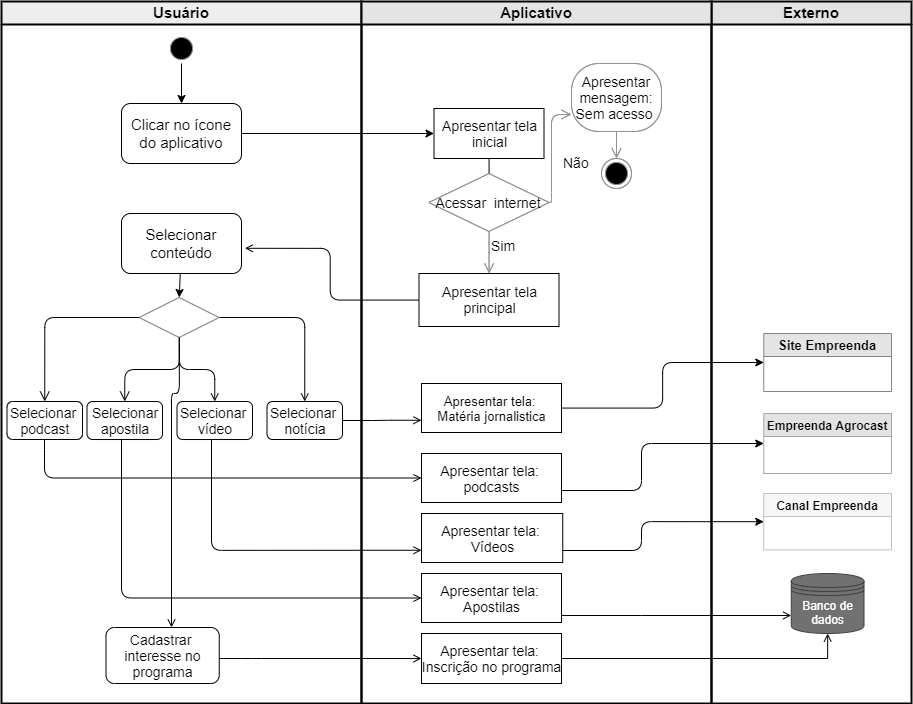
\includegraphics[scale=0.6]{Imagens/diagrama_aplicativo.png}
\fonte{O autor}
\label{figura_diagrama}
\end{figure}


\subsection{Conversão dos Conteúdos em um Aplicativo para Smartphone}

Para o desenvolvimento desta aplicação mobile, o projeto foi constituído de três fases: 

\begin{itemize}

\item{A Fase I - A Fase I correspondeu ao levantamento de necessidades, ou seja, à prospecção de indicadores importantes e necessários à promoção das competências empreendedoras que resultassem em promoção da cultura empreendedora nos alunos, assim como a assimilação dos conteúdos pertinentes ao surgimento de novos negócios rurais em Sergipe. Concomitantemente, ocorreram reuniões para planejamento das alternativas de implementação, com a participação dos organizadores do programa e tempo de programação;}

\item{Na Fase II ocorreram os encontros presenciais entre os profissionais especializados e os alunos participantes do Empreenda Agro Sustentável, ou seja, foi o momento em que todos os módulos de conteúdos pertencentes ao aplicativo foram abordados;}

\item{A Fase III consistiu no ciclo de desenvolvimento da programação lógica do aplicativo. À medida que se produzia os conteúdos presenciais, simultaneamente eram liberados os materiais digitais em forma de Mínimos Produtos Viáveis na plataforma, de modo que fosse possível a assimilação eficaz dos conteúdos pretendidos, assim como, realizar testes da aplicação com os usuários.}

\end{itemize}

\subsection{Método de Desenvolvimento da Aplicação}

Para o desenvolvimento do “software” foi adotado o método Scrum para a criação e a integração da aplicação desenvolvida e os conteúdos a serem disponibilizados \cite{schwalbe_scrum_2017}. O método consiste na concentração de esforços nas estratégias de execução de produtos complexos, lidando com uma forma de gerir projetos a partir de um ciclo de vida enxuto e repetitivo \cite{bernardo_framework_2019}. Os passos aplicados no método estão descritos na Figura \ref{figura_47}.

As funcionalidades do aplicativo a serem implementadas foram mantidas em uma lista que é conhecida como “Product Backlog”. No início de cada “Sprint”, era realizada uma “Sprint Planning Meeting”, ou seja, uma reunião de delineamento na qual eram priorizados os itens a serem desenvolvidos, e a equipe selecionava as atividades que eram compreendidas como capazes de serem implementadas durante o sprint \cite{trainning_education_services_curso_2018}.

\begin{figure}[H]
\centering
\caption{\textbf{Framework de gerenciamento do projeto Aplicativo Empreenda Agro Sustentável }}
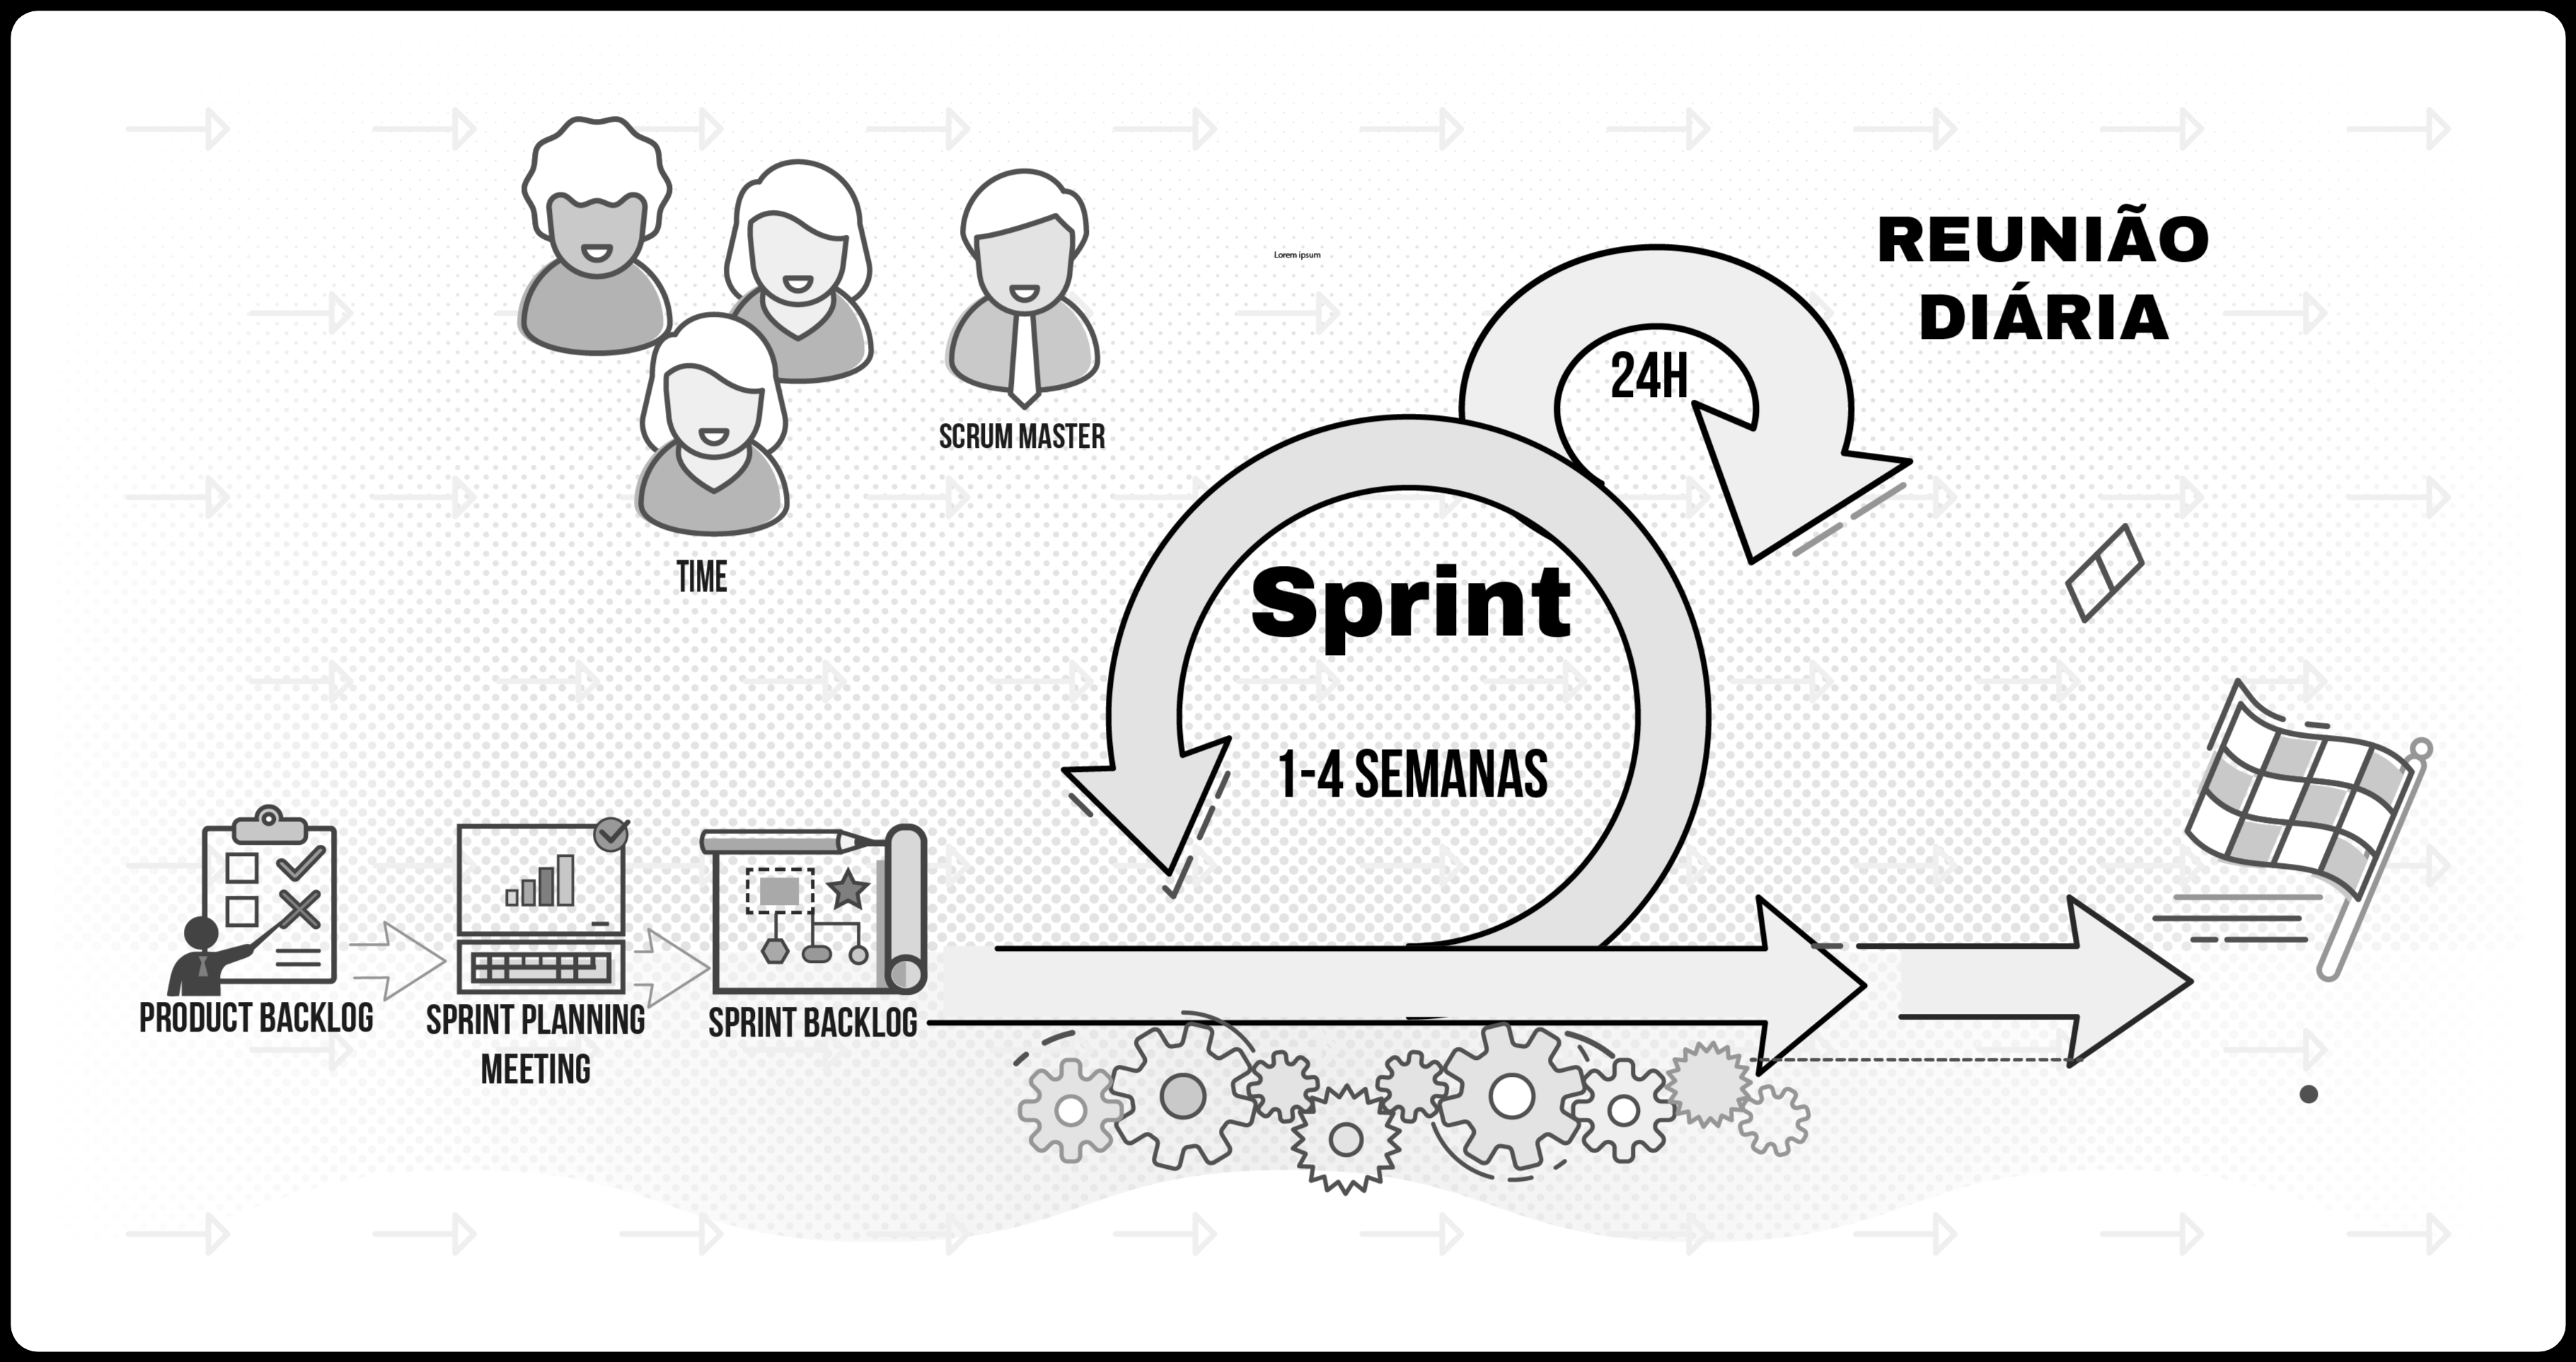
\includegraphics[scale=0.1]{Imagens/scrum.png}
\fonte{Adaptado de \citeonline{trainning_education_services_curso_2018}}
\label{figura_47}
\end{figure}

O software para aplicativos móveis, denominado Empreenda Agro Sustentável, foi desenvolvido na linguagem Kotlin \cite{smyth_kotlinandroid_2017}, no ambiente de programação Android \cite{android_conheco_2019}. O Android foi selecionado como sistema operacional, pois, domina o mercado móvel global em 2020, sendo instalado em 86,6\% de todos os “smartphones” em todo o mundo e espera-se que chegue até o ano de 2023 presente em 87,1\% dos aparelhos mundiais \cite{idc_idc_2020}.

O aplicativo foi projetado para ser compatível com a maioria das versões do Android a partir do nível 9 da API, ou seja, o Android 2.3. Isso significa que o aplicativo funciona em 99,7\% dos dispositivos móveis usando o sistema operacional Android em todo o mundo. Também foi projetado com um “design” adaptável, para ser compatível com qualquer “tablet” ou “smartphone”. Os conteúdos presentes no aplicativo, além da avaliação dos profissionais das áreas, foram também validados a partir das informações presentes na literatura acerca de assuntos sobre empreendedorismo e inovação para o meio rural, \cite{melo_sebrae_2008,oliveira_perfil_2006}.


Durante o desenvolvimento do programa Empreenda Agro Sustentável, foram realizados testes de usabilidade e confiabilidade do aplicativo Empreenda Agro sustentável pelos participantes do programa durante as oficinas de trabalho, com o intuito de observar o desempenho técnico do aplicativo e identificar problemas de navegação quando baixados em vários telefones Android. Alguns testes realizados foram: acesso a abas; abertura de links resultantes de dados externos; leitura dos materiais disponíveis em .PDF; acesso livre aos conteúdos disponíveis em vídeos (nenhum limite foi definido para a quantidade de dados a serem registrados no aplicativo) e navegação geral do ‘software’. Qualquer falha de acesso aos dados ou tempo de atraso na resposta do aplicativo, transição entre telas, uso do menu lateral, e dos botões da tela do aplicativo foram monitorados. Os comentários foram coletados por meio do módulo Android Vitals da plataforma Google Play Console.

Um questionário contendo perguntas para avaliação do aplicativo foi disponibilizado ao final do programa utilizando o método de divulgação 'Mobile Push Notifications' pela plataforma \textit{OneSignal}, para que fosse possível avaliar o desempenho do aplicativo. No questionário enviado continham perguntas tais como: “O menu lateral funciona bem? (SIM ou NÃO)”, “a tela inicial desliza bem? (SIM ou NÃO)”, “Você gostou do aplicativo? (SIM ou NÃO)”. Nas quais os usuários selecionavam o botão que contém a resposta que entendia ser a aceitável.







